%----------------------------------------------------------------------------
\chapter{Teljesítményelemzés és optimalizálás}
%----------------------------------------------------------------------------

(3-4 oldal)

Derp derp, valami szöveg. Árvíztűrő tükörfúrógép.

Selenium tesztek


%----------------------------------------------------------------------------
\section{Kollaborációs teljesítményelemzés}
%----------------------------------------------------------------------------


%----------------------------------------------------------------------------
\subsection{Szimuláció}
%----------------------------------------------------------------------------
A szimuláció célja automatizálni a felhasználói bemenetet egy teljesítmény méréshez. A megoldásnak tartalmaznia kell alapszintű felhasználói bemenet szimulálását: egérkattintás, szövegbeírás, várakozás és mivel egy grafikus modellt akarunk szerkeszteni a ``drag and drop'' funkcióra is szükség van. 

A böngészőautomatizálás Selenium Webdriver segítségével történt, ez az eszköz lehetővé teszi, hogy különböző nyelveken megírt (Python, Java, PHP stb. ) teszt esetekben a Webdriver API-val kommunikálva böngésző példányokat lehet irányítani. 
Seleniumhoz tartozik egy grafikus fejlesztőkörnyezet is ami Selenium IDE néven Firefox böngészőkiegészítésként fut, vele rögzíteni lehet felhasználói bemenetet és egér eseményeket, majd egy ilyen felvételt újralejátszani, módosítani. Ez előnyös teszterek számára akik repetitív munkát végeznek és nem tudnak programozni, de fejlesztők számára is jó, mert ezekből a felvételeket Python, Ruby stb teszteseteket lehet exportálni. 
Azon kívül, hogy automatizált tesztelésre a szkriptek alkalmasabbak, a Selenium IDE sajnos nem tud egérmozgatást rögzíteni, így nem hasznos a feladat szempontjából. A Selenium API javascript implementációját példáúl a selenium-webdriver csomag valósítja meg, viszont hamarosan kiderült, hogy ez a csomag nem támogatja ``drag and drop'' funckciót, emiatt a Python implementációt választottam. 

A fejlesztés korábbi stádiumában meg kellett győződni, hogy az alkalmazás valamennyire tűri a rossz internetkapcsolatot, ezért egy teszt környezetet alakítottam ki amiben két felhasználót szimulálva két selenium szkript ugyanazt a dokumentumot szerkeszti és véletlenszerű változtatásokat hajt végre a diagramon, pontosabban véletlen entitást mozgat el véletlen irányba. Az elvárt eredmény az, hogy rossz internet kapcsolat mellett is sok idő elteltével ugyanazt a diagramot látja a két felhasználó és azt, hogy ``ugyanazt'' a diagramot látják a diagram hash megegyezése igazolja.
 

\begin{figure}[!ht]
\centering
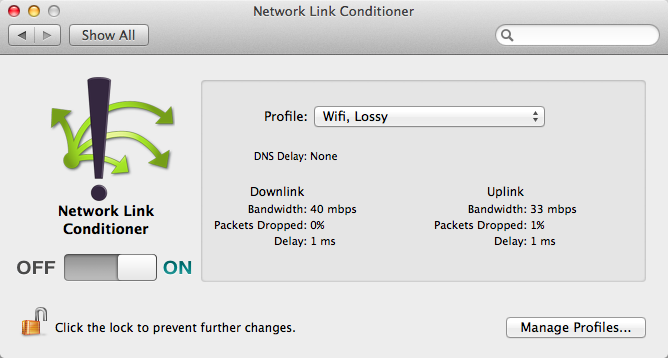
\includegraphics[width=15cm,keepaspectratio]{figures/nlc.png}
\caption{OSX Network Link Conditioner}
\label{fig:nlc}
\end{figure}


A rossz internet kapcsolat szimulálásához OSX-en a Network Link Conditioner alkalmazást használtam, ami az XCode fejlesztőkörnyezet egy kiterjesztése. A felhasználói felülete elég egyszerű és maximálisan megfelel a funkcionalitása a szimulációhoz, ezen kívül a létező profilok is hasznosak, ha példáúl egy gyenge jelű 3G kapcsolatot akarunk szimulálni. A paraméter amire kiváncsi voltam az a csomagvesztési arány volt, úgy azt kezdtem állítani egyre magasabb értékre. Az eszköz bekapcsolása után a ping parancssoros eszköz segítségével egy publikus ip-t pingelve\footnote{példáúl \lstinline{ping www.google.com}} kipróbáltam, hogy valóban akkora a csomagvesztés.

Az eredmény meglepő volt: már olyan csomagvesztési aránynál, ami nekem kicsinek tűnt, példáúl 10-20\% ?????nem lehetett bongeszni????
de a diagram egyezett a két felhasználónak. Wireshark protokolanalizátor segítségével megvizsgáltam, hogy ez miért is lehet, hogy nem veszett el esemény:


\begin{figure}[!ht]
\centering
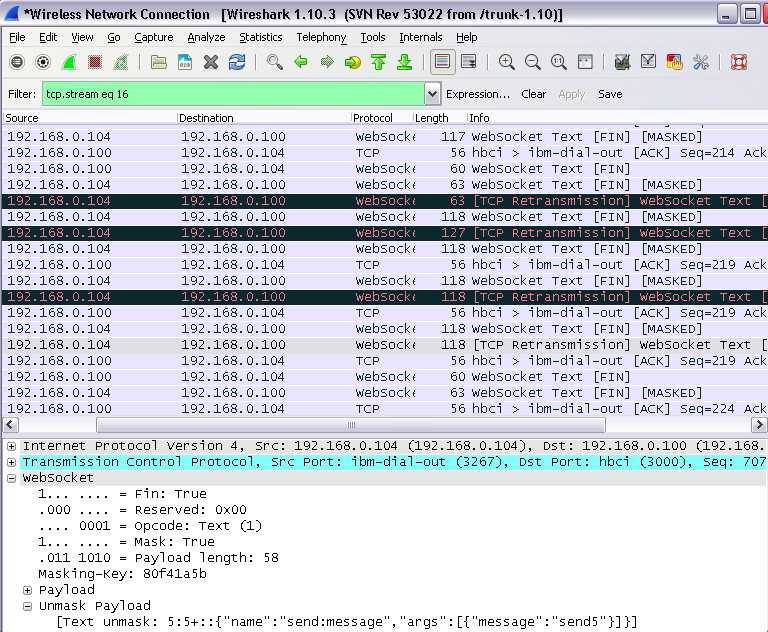
\includegraphics[width=15cm,keepaspectratio]{figures/wireshark.png}
\caption{A Websockets forgalom vizsgálata Wireshark segítségével}
\label{fig:wireshark}
\end{figure}


Wireshark-ban a Websockets protokoll-ra filtereltem, és egy újraküldött csomagra kattintva (a fekete sorok egyike) megnéztem az adott TCP folyamot. Látszik, hogy 192.168.0.104 -- a kliens ebben az esetben -- websockets üzeneteket küld, és a szerver TCP nyugtát küld (ACK) és amikor ez nem történik meg, akkor újraküldődik az üzenet.



++++++++++++++++++++++++
random módon két ember crudol és le kell mérni , hogy mennyire valószínű, hogy elvésznek a bemenetei
++++++++++++++++++++++++

%----------------------------------------------------------------------------
\section{Kliens oldali teljesítményelemzés}
%----------------------------------------------------------------------------
Derp.

A deep watching teljesitmenyelemzése

%----------------------------------------------------------------------------
\section{Webszerver teljesítményelemzés}
%----------------------------------------------------------------------------
Derp.

%----------------------------------------------------------------------------
\section{Adatbázis teljesítményelemzés}
%----------------------------------------------------------------------------

Vizsgáljuk meg, hogy csupán az adatbázis szint hogy viselkedik a terhelés szempontjából. Két kollekció van a dokumentumok és az entitások kollekciója. MongoDB shellből megvizsgálva a kollekcióimat vissza is igazolódik amit sejtettem, hogy a kollekciókon van indexállomány az elsődleges kulcson. A mongoDB shell az majdnem egy NodeJS shell, csak az adatbázis műveletei szinkronok és néhány nem-Javascript parancsot is támogat, példáúl:

\begin{itemize}
\item \lstinline{show dbs} -- az adatbázisok listázása
\item \lstinline{use <db> } -- adatbázis kiválasztása  
\item \lstinline{show collections} -- kollekciók listázása
\item \lstinline{show users} -- adatbázis felhasználók listázása
\end{itemize}

\begin{lstlisting}[caption=A diagram kollekció indexei]
> db.docs.getIndexes()
[
    {
        "v" : 1,
        "key" : {
            "_id" : 1
        },
        "ns" : "mint.docs",
        "name" : "_id_"
    }
]
\end{lstlisting}

Mivel a kliensoldali alkalmazás azonosító -- vagy elsődleges kulcs -- alapján kérdezi le a diagramokat, fölösleges ezzel a kollekcióval kezdeni az elemzést. Érdekesebb az \lstinline{entities} kollekció, ott nem azonosító alapján történik a lekérdezés, amikor egy diagramhoz a tartalmazott entitásokat kérjük.
Nézzünk meg egy ilyen lekérdezést a MongoDB shellben:

\begin{lstlisting}[caption=Az diagram kollekció egy lekérdezésének a query terve]
> db.entities.find({document:"52a37e129deb89c9bd0678aa"}).explain()
{
    "cursor" : "BasicCursor",
    "isMultiKey" : false,
    "n" : 200,
    "nscannedObjects" : 370,
    "nscanned" : 370,
    "nscannedObjectsAllPlans" : 370,
    "nscannedAllPlans" : 370,
    "scanAndOrder" : false,
    "indexOnly" : false,
    "nYields" : 0,
    "nChunkSkips" : 0,
    "millis" : 0,
    "indexBounds" : {

    },
    "server" : "Endres-Laptop-54.local:27017"
}
\end{lstlisting}


A [?] példában nem a lekérdezést lehet látni, hanem a lekérdezés tervet. Ez a terv sok fontos információval szolgál, ha optimalizálni akarunk:

[reference http://docs.mongodb.org/manual/reference/method/cursor.explain/]

\begin{itemize}
                        
  \item{cursor} - A kurzor típusa, amivel lefutott a query. Ha ez \lstinline{BasicCursor} akkor az adatbázis a teljes kollekciót beolvasta a query kiértékeléséhez, tipikusan akkor, ha nem tudott semmilyen indexet felhasználni a lekérdezéshez.
  \item{isMultikey} -  Olyan mezőket is lehet indexelni, aminek az értéke egy tömb. Példáúl \lstinline|{a: 1, b : [1,2,3,4]}| dokumentumok esetében lehetséges a \lstinline{b} tömb elemeit is indexelni. 
  \item{n} - A találatok száma. A fenti példában ez 200.
  \item{nscanned} - A dokumentumok száma ami meg lett vizsgálva, a query kiértékeléséhez. Arra kell törekedni, hogy a \lstinline{n} és a \lstinline{nscanned} közel legyenek egymáshoz. A fenti példában ez 370.

   \item{scanAndOrder} - Ez akkor \lstinline{true}, ha az adatbázis nem tudta felhasználni az indexet rendezésre és a találatokat újra kelett rendezni.
   \item{indexOnly} - Lehetséges olyan indexet felépíteni -- compound index -- ami több attribútumra vonatkozik egyszerre és ha az összes attribútuma a találatoknak benne volt az indexben, akkor az index ``fedi'' a queryt és csak az index alapján értékelődött ki. 
   \item{nYields} - A lekérdezés során hányszor kellett feloldani az olvasás zárat ahhoz, hogy egy másik írás query megtörténhessen. 
   \item{millis} - A lekérdezéshez szükséges ezredmásodpercek száma.


\end{itemize}

Amikor 370 rekord van a kollekcióban akkor elég gyorsan lefut a lekérdezés, gyakorlatilag azonnal, de vizsgáljuk meg hogy alakul ez amikor több rekord van és ugyanazt a 200-at kérdezzük le:


\begin{table}[H]
\centering
\begin{tabular}{|c|c|}

%content goes here
\hline
Rekordok száma & Lekérdezési idő ezredmásodpercben \\
\hline
370 & 0 \\
2000 & 0 \\
20000 & 11 \\
200000 & 89 \\
500000 & 220 \\
1000000 & 447 \\
2000000 & 907  \\
\hline
\end{tabular}
\caption{Lekérdezési idő alakulása az összes rekord száma szerint } 
\end{table}

Látszik, hogy elég sok rekordnál, egy diagram elemeinek lekérdezése már másodperc nagyságrendű időbe telik. Ez még tolerálható lehetne, mert 10000 felhasználóig valószínüleg 2000000 alatt maradna az összes entitás száma és a lekérdezések nagy része úgyis elsődleges kulcs alapú -- ami gyors. A 10000-es nagyságrendet meghaladva felhasználó számban (feltéve, hogy átlagban egy felhasználó 100 elemet hoz létre összesen) már túl lassúnak bizonyulna ez a megoldás.

Megvizsgáltam mennyire hatékony lehet a megoldás erre a próblémára, nyilvánvalóan indexelni kell a \lstinline{document} attribútumás az entitás kollekciónak és ez a következőképpen történik a MongoDB shellben:

\begin{lstlisting}[caption=Index létrehozása]
> db.entities.ensureIndex({document: 1})
> db.entities.getIndexes()
[
    {
        "v" : 1,
        "key" : {
            "_id" : 1
        },
        "ns" : "mint.entities",
        "name" : "_id_"
    },
    {
        "v" : 1,
        "key" : {
            "document" : 1
        },
        "ns" : "mint.entities",
        "name" : "document_1"
    }
]
\end{lstlisting}

A \lstinline{getIndexes()} paranccsal ellenőriztem, hogy tényleg létre is jött az index. Újból \lstinline{.explain()}-vel indítva lekérdezést a query tervben látszik, hogy \lstinline{"cursor" : "BtreeCursor document_1"}, tehát már az új indexet használja fel a kereséshez, ráadásul, a megvizsgált rekordok száma megegyezik a találatok számával. 

Nem meglepő, hogy 2000000 rekord esetén is majdnem egy másodperc helyett -- index segítségével -- 0 ezredmásodpercet jelez a query terv. Azt is meg lehet vizsgálni, hogy ez a kényelem mennyibe kerül és ezt a \lstinline{db.entities.stats()} paranccsal lehet megtudni:

\begin{lstlisting}[caption=Kollekció és index nagysága]
> db.entities.stats()
{
    "ns" : "mint.entities",
    "count" : 2000370,
    "size" : 208047512,
    "avgObjSize" : 104.00451516469454,
    "storageSize" : 243314688,
    "numExtents" : 13,
    "nindexes" : 2,
    "lastExtentSize" : 68579328,
    "paddingFactor" : 1.0000000000000022,
    "systemFlags" : 1,
    "userFlags" : 0,
    "totalIndexSize" : 177672656,
    "indexSizes" : {
        "_id_" : 64917440,
        "document_1" : 112755216
    },
    "ok" : 1
} 
\end{lstlisting}

Ebből kiderül, hogy 200MB az adat mérete és emellett az index mérete 178MB, tehát az összes tárhely majdnem a felét a két index foglalja el. Ennek az a magyarázata -- többek között -- hogy kevés adatot tárolunk egy rekordban, ami az \lstinline{avgObjSize} eredmény szerint 100 bájt. Az entitásokat kibővítve új adatokkal, példáúl színnel, szerencsére nem fog nőni az index mérete és kedvezőbb lesz a tárfoglalási arány.


